\documentclass[tikz,border=12pt]{standalone}
% Match the sans-serif font stack used by the Minimal Mistakes site theme.
% TeX Gyre Heros is the TeX-compatible Helvetica implementation.
\usepackage[T1]{fontenc}
\usepackage{tgheros}
\renewcommand{\familydefault}{\sfdefault}

\usepackage{amssymb}
\usetikzlibrary{arrows.meta,calc,positioning}

\definecolor{coral}{HTML}{FA5252}
\definecolor{ink}{HTML}{343A40}

\begin{document}
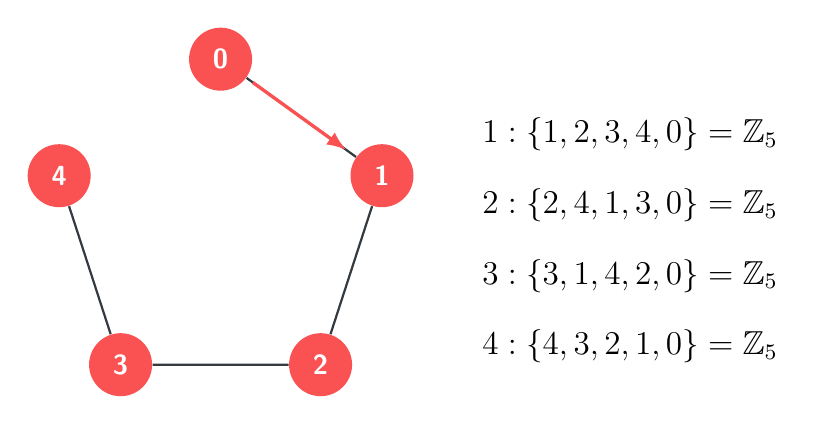
\begin{tikzpicture}[
  element/.style={circle, fill=coral, text=white, minimum size=8mm, inner sep=0pt, font=\bfseries},
  edge/.style={ink, line width=0.8pt},
  steparrow/.style={-{Latex[length=2.5mm]}, coral, very thick}
]
  \node[element] (z0) at (0,2.2) {0};
  \node[element] (z1) at (2.05,0.72) {1};
  \node[element] (z2) at (1.27,-1.68) {2};
  \node[element] (z3) at (-1.27,-1.68) {3};
  \node[element] (z4) at (-2.05,0.72) {4};

  \draw[edge] (z0) -- (z1) -- (z2) -- (z3) -- (z4) -- cycle;
  \draw[steparrow] ($(z0)!0.2!(z1)$) -- ($(z0)!0.78!(z1)$);

  \node[anchor=west, font=\large] at (3.2,1.25) {$1: \{1,2,3,4,0\}=\mathbb{Z}_5$};
  \node[anchor=west, font=\large] at (3.2,0.35) {$2: \{2,4,1,3,0\}=\mathbb{Z}_5$};
  \node[anchor=west, font=\large] at (3.2,-0.55) {$3: \{3,1,4,2,0\}=\mathbb{Z}_5$};
  \node[anchor=west, font=\large] at (3.2,-1.45) {$4: \{4,3,2,1,0\}=\mathbb{Z}_5$};
\end{tikzpicture}
\end{document}
